\documentclass[a4paper, 10pt]{scrartcl}

\title{MSE OrdDiff}
\subtitle{Formulary}
\author{ssteiner}
\date{\today}
\usepackage[T1]{fontenc}
\usepackage[UTF8]{inputenc}

% Mathematik-Pakete
\usepackage{amsmath}
\usepackage{amssymb}
\usepackage{amstext}
\usepackage{amsfonts}
\usepackage{mathrsfs}
\usepackage{paralist}
\usepackage[pdftex]{graphicx}
\usepackage{colortbl}
\usepackage[table]{xcolor}
\usepackage{hyperref}
\usepackage{multicol}
\usepackage{tabularx}
\usepackage{booktabs}
\usepackage{siunitx}
\usepackage{ltablex} %to combinate longtable and tabularx
\usepackage{bm}
\usepackage{arydshln} % hdashline

	%title
	\makeatletter         
	
	\def\@maketitle{   % custom maketitle 
		

		\centering{\LARGE \bf \textsf{\@title}} 
		\smallskip \\
		\centering{\large \bf \textsf{\@subtitle}} 
		\smallskip \\
		\centering{ \bf \textsf {\@author}}
		\medskip \\
		\centering{\bf \textsf{ \@date }}
		\smallskip \\
		\noindent\rule{\textwidth}{0.5pt}
		\smallskip
	}
	\makeatother

\usepackage[automark]{scrlayer-scrpage}
\clearscrheadings
\clearscrplain
%header footer

\pagestyle{scrheadings}
\lohead{\pagemark \hspace{0.3cm }  \textcolor{gray}{\rule{0.25cm}{0.25cm}} \hspace{0.3cm } \leftmark }
\cohead{}
\rohead{}
\setheadsepline[1.3\textwidth]{0.02cm} 

\rofoot{}
\cofoot{}
\lofoot{}






%si units
\sisetup{sticky-per=true,per-mode=symbol}


%geometry
\usepackage[a4paper]{geometry}
\geometry{verbose,tmargin=1.5cm,lmargin=2cm,rmargin=2cm,bmargin=3cm}


\usepackage[english, ngerman]{babel}
\setlength{\parindent}{0cm}
%font
\usepackage{lmodern}

	
	

	
	
	


\definecolor{darkgreen}{RGB}{0,100,0}
\definecolor{lightgray}{gray}{0.9}

\renewcommand{\arraystretch}{1.2}

\newcommand{\dx}{\hspace{2pt}dx}
\newcommand{\dd}[1]{\hspace{2pt}d#1}
\newcommand{\laplace}{\Delta}
\newcommand{\qed}{\begin{flushright}
		$\blacksquare \dagger$ \end{flushright}}
%vektor
\newcommand{\ve}[1]{\textbf{#1}}

\begin{document}
	\maketitle 

	\setlength{\parskip}{0cm}
	\setcounter{tocdepth}{1}	

	\tableofcontents 	
	
	\smallskip 
	\rule{\textwidth}{0.5pt}
	\smallskip
	\keepXColumns %ltablex
	
\section{Modellbildung}
\begin{tabularx}{\columnwidth}{p{2.8cm}XX}
	\hline 
	\multicolumn{3}{c}{\textbf{Grundbegriffe}}\\
	Diffgleichung n-ter Ordnung & $F(x,y,y',y'',\dots, y^{(n)}) = 0$ & 
	Intervall: $I\subseteq R$ \newline 
	Bereich: $\Omega \subseteq I \times \mathbb{R}^{n+1}$ \newline stetige Funktion $F: \Omega \rightarrow \mathbb{R}$ \\
	\hline 
	explizite  DGL &$y^{(n)} = G(x,y,y',y'',\dots,y^{(n-1)}$ & nach $y^{(n)}$ aufgelöst\\
	implizite DGL & nicht nach $y^{(n)}$ aufgelöst & \\
	\hline 
	Lösung von DGL & n mal differenzierbare Funktion &$\forall x\in I$ \\
	
	 & Lösen einer DGL gibt eine allgemeine Lösung & Lösen eines Anfangswertproblems/Randewrtproblems ergibt  spezielle, partikuläre Lösung\\
	Anfangswertproblem & $\begin{cases}
		F(x,y,y',y'',\dots, y^{(n)}) & = 0,\quad  (x,y,\dots,y^{n}) \in \Omega \\
		y(x_0)  &= y_0\\
		y'(x_0) &= y_1\\
				&\vdots \\
						y^{n-1}(x_0) &= y_{n-1}\\
	\end{cases}$& 
	\\
	Randwertprobleme & \multicolumn{2}{p{14cm}}{andere Phänomene als bei Angfangswertproblemen, Existenz- und Eindeutigkeitsaussagen für AWPs nicht mehr}\\
	\hline 
	\multicolumn{3}{c}{\textbf{Klassifikation}}\\
	linear & $a_n(x)\cdot y'(n) + \cdots + a_1(x)\cdot y' + a_0(x)\cdot y = g(x)$ & $a_i(x)$: fest vorgegebene funktionen\\
	homogen & $g(x) = 0 \quad \forall x\in I$ & $g(x)$: Störfunktion, Ihomogenität \\
	konstante Koeffizienten & $a_n\cdot y'(n) + \dots + a_1\cdot y' + a_0\cdot y = g(x)$  & $a_i$: konstante Koeffizienten, $a_n\neq 0$\\
	\multicolumn{3}{c}{spezialfälle 1. Ordnung}\\
	linear & $y' = f(x)\cdot y + g(x) $ & \\
	Exakte DGL & $M(x,y) + N(x,y)\cdot y'(x) = 0$ & Bedingung: $M_y(x,y) = N_x(x,y)$\\
	separierbar & $y' = g(x)\cdot h(y)$ & \\
	autonom & $y' = f(y)$ & autonom $\subseteq$ separierbar, $ g(x) = 1$  \\
	Typ unbestimmtes Integral & $y' = g(x)$ & separierbar aber nicht autonom\\
	\hline 
	\multicolumn{3}{c}{\textbf{Systeme von Differentialgleichungen}}\\
	
	System von DGL 1. Ordnung & 
	\multicolumn{2}{p{14cm}}{ $\begin{matrix} y_1' &=& f_1(x,y_1,\dots,y_n) \\ \vdots & &\vdots \\ y_n' &=& f_n(x,y_1,\dots,y_n)\\\end{matrix} \qquad $ 
	$\bm{y}(x) = \left(\begin{matrix} y_1(x) \\ \vdots \\ y_n(x)\end{matrix} \right) , \quad
	\bm{f}(x, \bm y) = \left(\begin{matrix} f_1(x,\bm y) \\ \vdots \\ f_n(x, \bm y)\end{matrix} \right)$}\\
	vektorielle Schreibweise & $\bm y' = \bm f(x,\bm y)$ & \\
	
	Anfangswertproblem & $\begin{cases} \bm y' & = \bm f(x,\bm y),\quad (x,\bm y)\in \Omega\subseteq \mathbb{R}\times\mathbb{R}^n \\ \bm y(x_0) &= \bm y_0\end{cases}$ & \\
	\hline
	\multicolumn{3}{c}{\textbf{Richtungsfeld}}\\
	$y'=F(x,y)$&
	DGL ,$n=1$, explizit: jedem Punkt $(x,y)$ wird ein Steigungswert zugeordnet ergibt Richtungsfeld & 
	 \raisebox{-.8\totalheight}{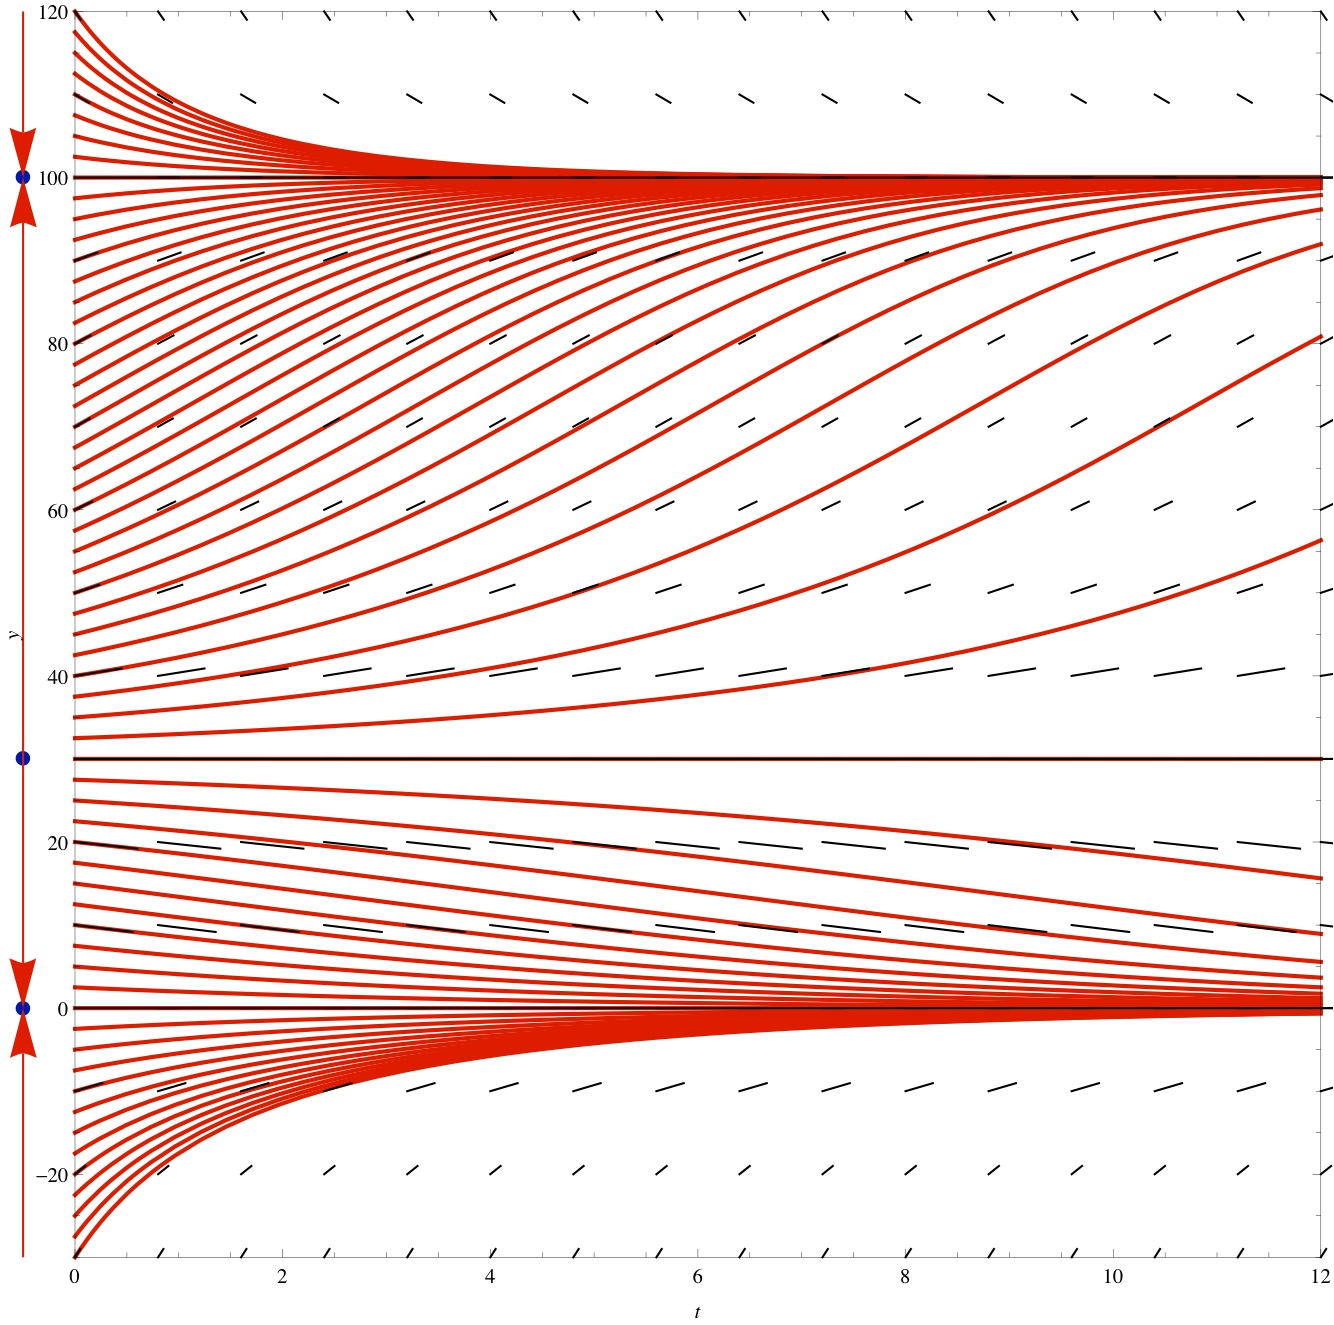
\includegraphics[scale = .15]{images/richtungsfelder}}\\
	Typ unbestimmtes Integral & Richtungsfeld y- unabhängig & \\
	autonome DGL & Richtungsfeld x-unabhängig & \\
	\hline 
	\multicolumn{3}{c}{\textbf{Lösbarkeit}}\\
	Lipschitz-Stetigkeit & $|\bm f(x,\bm y_1) - f(x,\bm y_1)| \leq L|\bm y_1 - \bm y_2|$ & $f(x,\bm y)$ muss stetig sein und Libschitz-Stetigkeit erfüllen für Eindeutigkeit\\
	Erüfllt wenn & 	 $\dfrac{\partial \bm f(x,\bm y_i)}{\partial y_i}$ stetig ist & \\
	Piccard-Lindelöf &\multicolumn{2}{p{14cm}}{ offene Menge: $\Omega \subseteq \mathbb{R}\times \mathbb{R}^n $\newline
	zulässige Funktion$ \bm f:\Omega \rightarrow\mathbb{R}^n \quad (x,\bm y) \mapsto \bm f(x,\bm y)$\newline 
	beliebiger Punkt $  (x_0,\bm y_0)\in \Omega$ \newline 
	$\rho > 0$ hinreichend klein $\bm y(x): [x_0-\rho,x_0+\rho] \to \mathbb{R}^n \Rightarrow$ \newline 
	dann existiert genau eine Lösung }\\
\end{tabularx}

	\section{Gewöhnliche Differentialgleichung}
\renewcommand{\arraystretch}{2.5}
\begin{tabularx}{\columnwidth}{p{2.8cm}XX}
	 \hline 
	\multicolumn{3}{c}{\textbf{Analytische Verfahren}}\\
	
	\hline 
	\multicolumn{3}{c}{DGL 1. Ordnung}\\
	\hdashline
	Separierbare DGL & 
	$\begin{cases} y' &=g(x)h(y) \quad  h(y_0)\neq 0\\ y(x_0) &= y_0  \end{cases}$ & 
	$\int\limits_{y_0}^y \dfrac{1}{h(\tilde y)}d\tilde y = \int\limits_{x_0}^x g(\tilde x)d\tilde x$\\
 
	\hdashline
	Substitution  & $y' = A\left(\dfrac{y}{x}\right) = A(u) \quad u(x) = \dfrac{y}{x}$ & Rücksubstitution $y = x\cdot u(x)$\\
	\hdashline
	Lineare DGL & $y' = f(x)\cdot y + g(x) \qquad  y = y_h + y_s$ & $y_h$: homogene Lösung \newline $y_s$: partikuläre Lösung\\
	
	Linearität & \multicolumn{2}{p{13cm}}{Eine Linearkombination von verschiedenen Störfunktionen führt auf einen Ansatz entsprechender Linearkombinationen}\\
	Resonanz & \multicolumn{2}{p{13cm}}{Wenn die Störfunktion eine Lösung der homogenen DGL ist muss der \textbf{Ansatz mit $x$ multipliziert} werden}\\
	
	\textbf{Homogene $\mathbb{L}$} & $y_h = K\cdot e^{F(x)} \qquad F(x) = \int f(x)dx$ & \\
	\multicolumn{3}{c}{\textbf{Partikuläre $\mathbb{L}$}}\\				
	\cline{2-3}
	Ansatz durch Einsetzen &  
	Störfunktion g(x)\newline 
	$a\;(\text{const})$\newline 
	$a_0 + a_1x +\cdots +a_mx^m$\newline
	$ae^{\lambda x}$\newline
	$a\sin(mx)$\newline 
	$b\cos(mx)$\newline 
	$a\sin(mx) + b\cos(mx)$&
	Ansatz für $y_s(x)$  \newline 
	$b\;(\text{const})$ \newline 
	$b_0 + b_1x + \cdots + b_mx^m$\newline 	
	$be^{\lambda x}$\newline 			 
	$c\sin(mx) + d\cos(mx)$\\
	\cline{2-3}
	Variation \newline der Konstanten & $y_p = K(x)\cdot e^{F(x)} \qquad F(x) = \int f(x)dx$ & $K(x) = \int g(x)e^{-F(x)}dx$\\
	\hline
	\multicolumn{3}{c}{DGL n-ter Ordnung}\\
	\hdashline 
	linear, konstante Koeffizienten & $a_n\cdot y'(n) + \cdots + a_1\cdot y' + a_0\cdot y = g(x)$  & $a_i$: konstante Koeffizienten, $a_n\neq 0$\\
	Linearkombination & Jede Linearkombination von $\mathbb{L}$ ist wieder eine Lösung & $C_1y_1 + C_2 y_2 \in \mathbb L$\\
	Anzahl Lösungen & n linear unabhängige Lösungen & \\
	Homogene $\mathbb{L}$ & \multicolumn{2}{p{14cm}}{ $y = e^{\lambda x} \qquad P(\lambda) = \lambda^n +a_{n-1}\lambda^{n-1} + \cdots + a_1\lambda + a_0 = 0 \quad \lambda\in\mathbb{C}$}\\
	
	\multicolumn{3}{p{\columnwidth}}{$P(\lambda)$: m-fache reelle Nullstellen  $\lambda\in\mathbb{R} \qquad y_i=C_i x^{i-1}e^{\lambda x} \qquad  i=1, \dots,m$}\\
	
	\multicolumn{3}{p{\columnwidth}}{$P(\lambda)$: m-fache komlexe Nullstellen $\lambda\in\mathbb{C} \quad \lambda = \alpha\pm j\beta \qquad y_i = x^{i-1}e^{\alpha x}(C_i\cos\beta x + C_{m+i}\sin\beta x) \quad  i=1, \dots,m$} \\
	Partikuläre $\mathbb{L}$& \multicolumn{2}{p{14cm}}{Einsetzen eines Ansatzes, der dieselbe Form wie die Störfunktion hat mit unbestimmten Parametern}\\
	\hline 
	\multicolumn{3}{c}{\textbf{Numerische Verfahren}}\\
	\hdashline 
	Grundbegriffe & $x_k$: Näherungswerte ($k\in \mathbb{N}$)& $t_k$: Stützstellen ($k\in \mathbb{N}$)\\
	\hdashline
	\multicolumn{3}{c}{Einschrittverfahren}\\
	Schrittweite & $h = t_{k+1} - t_k$ (const.) & $t_k = t_0 + k\cdot h$\\
	explizite Verfahren & $x_{k+1} = \Psi_f(t_k,x_k,h) = x_k + h\cdot \Phi_k(t_k,x_k,h)$& $\Phi_f(t_k,x_k,h) = \dfrac{\Psi_f(t_k,x_k,h) -x_k}{h}$\\
	\hdashline 
	Explizites Euler Verfahren ($p=1$) & $\begin{cases} t_{k+1} &= t_k+h \\ x_{k+1} &= x_k + h\cdot f(t_k,x_k)\end{cases}$ & 
	$\Psi_f(t_k,x_k,h) = x_k + h\cdot f(t_k,x_k)$ \newline 
	$\Phi_f (t_k,x_k,h) = f(t_k,x_k)$\\
	\hdashline 
	Mittelpunktsregel ($p=2$) & $\begin{cases} t_{k+1} &=t_k + h \\ x_{k+\frac{1}{2}} & = x_k + \frac{h}{2}\cdot f(t_k,x_k) \\ x_{k+1} &=x_k + h\cdot f(t_k+\frac{h}{2},x_{k+\frac{1}{2}})	\end{cases}$ & 
	$\Phi_f(t_k,x_k,h) = f\left(t_k + \frac{h}{2}, x_k + \frac{h}{2}f(t_k,x_k)\right)$\\
	\hdashline
	Heun-Verfahren ($p=2$) & $\begin{cases}t_{k+1} &= t_k+h\\ m_1 &= f(t_k,x_k) \\ m_2 & = f(t_k+h,x_k+h\cdot m_1)\\ x_{k+1} &= x_k +\frac{h}{2}(m_1+m_2)\end{cases}$ &
	$\Phi_f(t_k,x_k,h) = \dfrac{1}{2}(f(t_k,x_k) + f(t_{k+1},x_k +h\cdot f(t_k,x_k))$\\
	\hdashline 
	Klassisches Runge-Kutta-Verfahren ($p=4$)& 
	$\begin{cases}t_{k+1} &= t_k + h\\ m_1 &= f(t_k,x_k)\\ m_2 &=f(t_k +\frac{h}{2},x_k + \frac{h}{2}m_1)\\ m_3 &=f(t_k +\frac{h}{2},x_k + \frac{h}{2}m_2)\\ m_4 &=f(t_k +h,x_k + h m_3)\\ x_{k+1} &= x_k + \dfrac{h}{6}(m_1 + 2m_2 + 2m_3 + m_4)\end{cases}$ & 
	$\Phi_f = \dfrac{1}{6}(m_1 + 2m_2 + 2m_3 + m_4)$\\
	\hdashline
	Implizites Euler-Verfahren & $\begin{cases} t_{k+1} &= t_k + h\\ x_{k+1} &= x_k + h\cdot f(t_{k+1}, x_{k+1})\end{cases}$\\
	\hline 
	\multicolumn{3}{c}{Fehler und Fehlerordnung}\\
	\hdashline 
	Kategorien & \multicolumn{2}{p{13cm}}{
	(1)   Datenfehler: Fehler bei Anfangsbedingungen $x_0 \neq x(t_0)$  \newline 
	(2)  Diskretisierungsfehler: Fehler durch Approximationsverfahren\newline
	(3) Rechenfehler: bei Durchführung des Algorithmus, Rundungseffekte}\\
	\hdashline 
	(1) Datenfehler & 
	$|x^{(1)}(t) - x^{(2)}(t)| \leq e^{L(t-t_0) |x_1-x_2}$&
	$f(t,x)$ erfüllt Lipschitz-Bedingung\newline $x^{(1)}(t),x^{(2)}(t)$, Lösungen\newline
	$x_1,x_2$  Anfangsbedingungen\\
	(2) Diskretisierungsfehler & lokaler Diskretisierungsfehler (LDE)  & $\tau_{k,h} = \dfrac{x(t_{k+1}) - x_h(t_{k+1};t_k,x(t_k))}{h}$\\
	 &globale Diskretisierungsfehler (GDE)&
	 $\max\limits_{0\leq k\leq n}|e_k| = \max\limits_{0\leq k\leq n}|x(t_k) - x_k|$\\
	 (3) Rechenfehler & $\tilde x_{k+1} = \tilde x_k + h\cdot \Phi_f(t_k,\tilde x_k,h) + r_k$ & $r_k$: Rundungsfehler\\
	 \hdashline
	 Konsistenz & $|\tau_{k,h}| \leq Ch^p\qquad  (h\to 0)$ & $C$: Konstante $(C\in\mathbb{R})$\newline $p$: Ordnung Verfahren\\
	 Konvergent & $\max\limits_{0\leq k\leq n} |e_k| \leq Ch^p \qquad (h\to 0)$ &\\
	  & \multicolumn{2}{l}{Konsitenz der Ordnung p $\implies$ Konvergenz der Ordnung p}\\
	 \hdashline 
	 totaler Rechenfehler & \multicolumn{2}{l}{$\max\limits_{0\leq k\leq n} |\tilde{e}_k| = \left( \underbrace{|x(t_0) - x_0|}_{Fehler (1)} + \sum\limits_{k=0}^{n-1} (h\cdot \underbrace{|\tau_{k,h}|}_{Fehler (2)} +  \underbrace{|r_k|}_{Fehler (3)}   \right) e^{L(t_n-t_0)}$}\\
	 \hline 
\end{tabularx} 

\renewcommand{\arraystretch}{2}
	\section{Systeme von Differentialgleichungen}
	\begin{tabularx}{\columnwidth}{p{3cm}XX}
		\hline 
		\multicolumn{3}{c}{\textbf{Lineare Syteme}}\\
	lineares System von DGL 1. Ordnung &		
	$\begin{matrix} \dot{x_1} &=& a_{11}x_1 &+&\dots&+&a_{1n}(t)x_n&+&b_1(t)\\ 
	                \vdots    & & \vdots    & &     & &\vdots      & &\vdots \\
	                \dot{x_n} &=& a_{n1}x_1 &+&\dots&+&a_{nn}(t)x_n&+&b_n(t)\\ \end{matrix}$&\\

	Matrix-Vektor Notation & $\bm{\dot x} = A(t)\bm x + \bm b(t)$ & \\
	allgemeine Lösung & $\bm x = \bm x_h + \bm x_s$ & \\
	\hdashline 
	Homogene $\mathbb L$ & \multicolumn{2}{p{14cm}}{$\bm{\dot x} = A \bm x$ besitzt n linear unabhängige Lösungen $\bm x_1,\dots, \bm x_n$. Diese Lösungsmenge nennt man Fundamentalsysem von Lösungen}\\
	Lösungsansatz & $\bm x_h = e^{\lambda t}\cdot \bm c \qquad \bm c = (c_1,\dots,c_n)^t \newline A\bm c = \lambda \bm c \qquad \bm c(A-\lambda I) = |A-\lambda I| = 0$ &
	$\lambda_i$: Eigenwerte von A \newline $c$: Eigenvektor von A\\
	
	Eigenwerte & \multicolumn{2}{p{14cm}}
	{(1) n linear unabhängige Reelle Eigenwerte: $\lambda_i \in \mathbb{R}\quad  \forall i$ \newline 
	 (2) mindestens ein Paar  von konjugiert komplexen Eigenwerten: $\lambda_i \in \mathbb{C}$\newline
	 (3) mehrfache Eigenwerte: $\lambda_i = \lambda_j$}\\
	(1) reeller EW & $\bm x(t) = e^{\lambda t}\bm c$ & \\
	(2) komplexer EW & $\lambda = \mu + j\nu \bm c = \bm a + j \bm b \newline \bm x(t) = e^{\lambda t}\bm c = e^{(\mu + j\nu )t}(\bm a + j\bm b)$ &
	 $\bm z_1(t) = e^{\mu t}(\bm a \cos(\nu t) - \bm b sin(\nu t))$\newline 
	  $\bm z_2(t) = e^{\mu t}(\bm a \cos(\nu t) + \bm b sin(\nu t))$\\
	(3) k-fach reelle EWs & 
	$\bm x_i(t) = e^{\lambda t} \bm p_{m-1}(t) \quad (2\leq m \leq k)$ & 
	$\bm p_m(t) = \begin{pmatrix} p_1^{m}(t) \\ \vdots \\ p_n^{m} (t) \\\end{pmatrix} \quad (0\leq m\leq k-1)$\\
	(3*) k-fach komplexe EWs & Kombination aus (2) und (3) &\\
	verallgemeinerter EV& $\bm p_i(t) = (t\bm v + \bm p^*) \qquad (A-\lambda I)\bm p^* =  \bm v$ & $\bm v$: schon gefundener EV $\bm p_{i-1}$\\
	
	Entkopplung & $A = TDT^{-1} \newline  D = \operatorname{diag} (\lambda_1, \dots, \lambda_n), \quad T = (\bm v_1,\dots,\bm v_n)$ \newline $\bm \dot x = A\bm x \implies T^{-1}\bm{\dot x} = DT^{-1}\bm x$& $A$: muss Diagonalisierbar sein\newline $\bm v_i$ Eigenwektoren\\
	Matrix-Exponential & $\bm x = e^{At}\bm x_0$ & $e^{At} = I + At + \dfrac{A^2t^2}{2!} + \dots = \sum\limits_{k=1}^{\infty}A^k\dfrac{t^k}{k!}$\\
	\hdashline
	Beziehung DGL höherer Ordnung &
	$x^{(n)} = f(t,x,\dot x, \ddot a, \dots, x^{n-1})\qquad \equiv$ & $\begin{matrix}
	\dot x_1 &=& x_2\\	\dot x_2 &=& x_3\\ \vdots & & \vdots \\ 	\dot x_n &=& f(t,x_1,x_2,x_3,\cdots,x_n)\\
	\end{matrix}$\\
	\hdashline 
	
	DGL n-ter Ordnung mit konst. koeffizienten & $ x^{(n)} + a_{n-1}x^{(n-1)} + \dots + a_1\dot x + a_0 x = 0$  \newline $\bm{\dot x} = A\bm x$ & 
	$A = \begin{pmatrix}
	0 & 1 & 0 & \dots & 0 \\ 0 & 0 & 1 & \dots & 0 \\ \vdots & \ddots &   & \ddots & \vdots \\ \dots &   & \dots & 0 & 1 \\ -a_0 & -a_1 &  \dots & -a_{n-2} & -a_{n-1}\\
	\end{pmatrix}$\\
	
			
	\end{tabularx}
	\newpage
	\section{Beispiele}
 

\begin{tabularx}{\columnwidth}{p{2.5cm} X}
	\hline 
	\multicolumn{2}{c}{\textbf{Gewöhliche Differentialgleichungen }}\\
	\multicolumn{2}{c}{1. Ordnung}\\
	Lösung durch Substitution & 
	$y' = A\left(\dfrac{y}{x}\right) = A(u) \quad \text{subst.}\quad u(x) = \dfrac{y}{x} \quad u' = \dfrac{x\cdot y'-y\cdot1}{x^2} = \dfrac{y'-u}{x} $ \newline 
	$y' = x\cdot u' +u = A(u)  \quad u' = \dfrac{A(u)-u}{x} \quad \text{separierbar!}$ \newline 
	$\boxed{\int\dfrac{du}{A(u) - u} = \int \dfrac{dx}{x}} \quad \text{Lösung der DGL für } u(x) \quad y = x\cdot u(x)$\\
	Anwendung Beispiel&
	$y' = \dfrac{y}{x} - \dfrac{x^2}{y^2} \quad A(u) = u - \dfrac{1}{u^2} \quad u' = \dfrac{A(u) - u}{x} = -\dfrac{1}{u^2\cdot x} $\newline 
	$-\int u^2 du = \int \dfrac{1}{x} \quad -\dfrac{u^3}{3} = ln|x|+C \quad y(x) = x \cdot u(x) = x\cdot (C -3\ln|x| )^{1/3}$
	
	
	\\
\end{tabularx} 

\end{document}